%****************************************************
%	CHAPTER 2 - Prototype Design
%****************************************************
\chapter{Prototype Design}
\label{ch:proto}
%====================================================
\section{Conventions Used}
\label{sec:proto.conventions}
Attitude conventions used for the dynamic equation derivations in the following Chapter: \ref{ch:dynamics} are briefly discussed here. Often these aspects relating to conventions are omitted or assumed commonplace. It's important to clearly and unambiguously define a standard set frames to avoid uncertainty in the kinematics. Rotation matrices and angles are included briefly for the sake of completeness but the focus is on \emph{contrast} between rotation and transformation operations. Both \cite{spacecraftattitutdequaternions} and \cite{rigidbodylecture} provide an in depth explanation of rotational matrices and DCM attitude representation if such concepts are unfamiliar to the reader.
%====================================================
\subsection{Reference Frames Convention}
\label{subsec:proto.conventions.frames}
%====================================================
\begin{figure}[htbp]
\centering
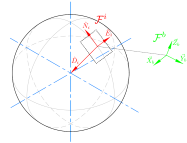
\includegraphics[width=0.6\textwidth]{figs/reference_frame}
\caption{Inertial and Body Reference Frames}
\label{fig:ref_frame}
\end{figure}
Regular aerospace (Euler) frames are used for principle inertial and body directions. Shown in Fig: \ref{fig:ref_frame}, the inertial frame,~$\mathcal{F}^i$, is aligned such that the $\vec{X}_i$ axis is in the $\hat{N}$orth direction, $\vec{Y}_i$ is in the $\hat{E}$ast direction and $\vec{Z}_i$ is  in the $\hat{D}$ownward direction\footnote{In orbital sequences this will be toward the Earths' center.}. The body frame, $\mathcal{F}^b$, then has both $\vec{X}_b$ and $\vec{Y}_b$ aligned with two perpendicular arms of the quadrotors' body and finally the $\vec{Z}_b$ axis pointing in the body's normal direction. The body frames axes are highlighted next in Sec:\ref{subsec:proto.conventions.motoraxis}. Frame superscripts $i$ and $b$ represent inertial and body frames respectively. Vector subscripts imply the reference frame inwhich that vector is measured with respect to. 
\par
The relative angular displacement between the two frames is commonly defined by the three angle Euler set, $[\phi ~\theta ~\psi]^T$. The Euler set represents rotations about the $\vec{X}$,$\vec{Y}$ and $\vec{Z}$ axes respectively. Depending on how the rotation sequence is formulated, those angles can 
\par
An inherent singularity does exists with such attitude representations. Indeed Quaternions are used later in Sec: \ref{subsec:dynamics.rigidbody.quaternion} in lieu of Euler angles, but they are easily understood and well suited to illustrate the distinction between rotation and transformation angles made here.
\par

\subsection{Motor Axis Layout}
\label{subsec:proto.conventions.motoraxis}
%****************************************************

%****************************************************
\section{Design}
\label{sec:proto.design}
%****************************************************
\subsection{Gimbal Articulation}
\label{subsec:proto.design.actuation}
%****************************************************
\subsection{Inertial Matrix Function}
\label{subsec:proto.design.inertia}
%****************************************************
\subsection{Overall Aspects}
\label{subsec:proto.design.aspects}
%****************************************************
\subsubsection{Vibration Damping}
%****************************************************
\subsubsection{Duct}
%****************************************************
\subsubsection{Landing Skids}
%****************************************************
\subsubsection{Motors \& ESCs}
%****************************************************

%****************************************************
\section{System Layout}
\label{sec:proto.layout}
%****************************************************
